\section{LTS synthesis from high-level MSCs\label{section:inductive-from-hMSC}}

Section \ref{subsection:inductive-synthesis-approach} discussed how system behaviors specified in collections of MSC scenarios can be first generalized as a system LTS, then decomposed as a set of agent LTSs. The QSM technique supports the incremental enrichment of an initial scenario collection through scenario queries. It also takes other models into account, such as goals, so as to preserve multi-view consistency. Behavior generalization, incremental synthesis and multi-view consistency were the three main requirements identified in Section \ref{subsection:inductive-synthesis-requirements}. 

When it is coupled with other synthesis techniques such as goal mining from scenarios\footnote{whose simplest form consists in asking ``why'' questions about negative scenarios.} \cite{Damas:2006}, interactive LTS induction appears really effective; starting from a small initial scenario collection, richer system models can be synthesized through a few iterations only. Chapters~\ref{chapter:evaluation} and \ref{chapter:tool-support} will illustrate this claim through evaluations and discussion of tool support.

For non-toy systems, however, large scenario collections might become unmanageable. In particular, the consistency of the collection might be difficult to guarantee without costly refactoring of scenarios. One notable reason is that all scenarios of a collection are required to start in the same system state; this may imply a lot of redundancy in the required input descriptions.

One way to tackle this problem is to use high-level message sequence charts (hMSCs) for structuring scenario descriptions. As detailed in Section \ref{subsection:background-hmsc}, hMSCs are directed graphs where each node refers to a MSC or a finer grained hMSC (see Fig.~\ref{image:train-hmsc}). Scenarios can then be structured by introducing scenario alternatives, sequencing and loops.

A structured form of scenario \emph{helps} specifying a large system with scenarios. It does not \emph{solve} the problem of achieving a complete and consistent view of agent behaviors:
\begin{itemize}
\item capturing all possible interleavings of a distributed system proves difficult with scenarios; a single hMSC is therefore hardly complete in practice;
\item complementary system features are to be specified in complementary models; in addition to multiple system views, specifying system behaviors in multiple hMSCs makes sense.
\end{itemize}

A synthesis technique for merging and generalizing behaviors described in hMSCs appears to be a convenient extension to the synthesis technique described in sections \ref{section:lts-induction-from-mscs} and \ref{section:inductive-mutliview-consistency}. To this end, the LTS synthesis statement is first revisited in Section~\ref{subsection:hmsc-induction-problem-revisited}. Our inductive algorithm is then adapted in Section \ref{subsection:hmsc-induction-algo-adaptation}.

\subsection{Revisiting the LTS synthesis statement\label{subsection:hmsc-induction-problem-revisited}}

Merging multiple hMSCs $H_1,\ldots,H_n$ with respect to trace behaviors amounts to compute the union of their respective languages. This is equivalent to building a new hMSC $H$ reaching the finer-grained $H_1,\ldots,H_n$ from its initial state. Additional positive scenarios $S^+_1,\ldots,S^+_n$, typically coming from scenario queries, may be integrated in a similar way. This is illustrated in Fig.~\ref{figure:multiple-hmscs}.

\begin{figure}\centering
\scalebox{.70}{
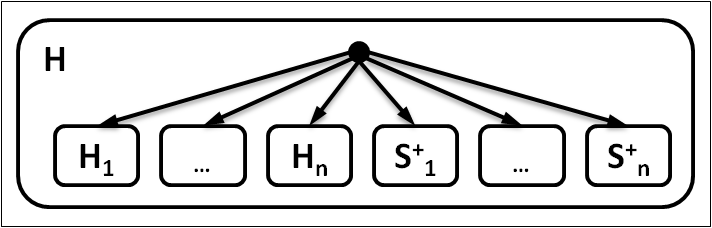
\includegraphics[trim=3mm 3mm 3mm 3mm, clip]{src/4-inductive/images/multiple-hmscs}}
\caption{Merging multiple hMSCs amounts to builds a new one that reaches finer-grained hMSCs from its initial state.\label{figure:multiple-hmscs}} 
\end{figure}

However, a hMSC only captures positive behavior examples. As explained in previous sections, negative information is needed for avoiding overgeneralization. Negative scenarios, fluents, goals, etc. all provide a source of negative knowledge that can be used to constraint the induction process. The algorithmic adaptations considered later stay compatible with the constraint mechanism based on equivalence relations on system states.

Without loss of generality therefore, we will assume that behaviors are specified through one hMSC only, complemented with a scenario collection. The latter contains negative scenarios and answers to scenario queries. Under these assumptions, the LTS synthesis statement is restated as follows: 

\begin{quote}
\underline{Given}~a hMSC $H$ and a scenario collection $Sc = (S^+,S^-)$ consistent with each other
\begin{align*}
[\mathcal{L}^+(Sc) \cup \mathcal{L}(H)] \cap \mathcal{L}^-(Sc) &= \emptyset
\end{align*}
\underline{Synthesize}~the system as a composition of agent LTSs
\begin{align*}
System = (Ag_1 \parallel \ldots \parallel Ag_n)
\end{align*}
\underline{Such that}~$H$, $Sc$ and $System$ are consistent.
\end{quote}

The hMSC trace semantics is left open in the formulation above. In other words, one has to decide which set of behaviors does $\mathcal{L}(H)$ denote. We recall below the relations between the three hMSC languages covered in Section \ref{subsection:background-hmsc}: 
\begin{align}
\mathcal{L}_{strong}(H) \subseteq \mathcal{L}_{weak}(H) &\subseteq \mathcal{L}_{arch}(H)
\end{align}

$\mathcal{L}_{strong}(H)$ denotes the set of system behaviors with strong sequential composition of hMSC nodes and total event ordering inside MSCs. It is the simplest and most intuitive model for stakeholders involved in early phases of system design. However, it supposes an implicit synchronization scheme used by the agents that is usually not available in real distributed systems. $\mathcal{L}_{arch}(H)$ is the most realistic for such systems, as it captures all possible interleavings of agent behaviors. $\mathcal{L}_{weak}(H)$ is mainly used for explaining and detecting implied scenarios in hMSC specifications \cite{Uchitel:2003}; it is also the hardest to compute.

Making a choice of semantics is required for generalizing behaviors because inductive synthesis takes a set of traces as input. The chosen semantics must of course fit domain assumptions. From an algorithmic point of view however, the three hMSC languages above require the same adaptations of the inductive process, as explained in the next sections.

\subsection{Generalizing high-level MSC languages\label{subsection:hmsc-induction-algo-adaptation}}

Recall that learning a regular language $L$ aims at generalizing a positive sample $S_+$ under the control of a negative sample $S_-$ such that the following relation of language inclusions holds:
\begin{align}
S_+~~\subseteq~~L~~\subseteq~~\Sigma^*\setminus S_-
\end{align}

LTS synthesis from a scenario collection $Sc$ reduces to grammar induction because the sets $\mathcal{L}^+(Sc)$ and $\mathcal{L}^-(Sc)$ are valid positive and negative samples, respectively (see Section \ref{subsection:inductive-lts-synthesis-reduction}). In particular, they denote \emph{finite} sets of traces.

When considering the generalization of hMSC behaviors, the sets of positive and negative traces are $\mathcal{L}^+(Sc) \cup \mathcal{L}(H)$ and $\mathcal{L}^-(Sc)$, respectively. The positive set is no longer a sample because $\mathcal{L}(H)$ might contain an infinite number of traces. Therefore, the current problem statement no longer fits exactly in the identification in the limit framework presented in Section \ref{section:inductive-background}. 

From a theoretical point of view, it means that generalizing hMSC languages is a different problem than generalizing MSC languages; therefore, further study would be needed to re-state the convergence criteria and the notion of characteristic sample in particular. From an algorithmic point of view, however, only a few adaptations of RPNI and QSM are required. They are explained in the next section.

\subsection{The Automaton State Merging algorithm\label{subsection:automaton-state-merging}}

The algorithm to generalize behaviors specified in a hMSC is given in Algorithm~\ref{ASM}, called Automaton State Merging (ASM). It is very similar to QSM, given in Section~\ref{section:lts-induction-from-mscs}, except that the interactive feature is ommited here (we discuss it later). QSM itself being an interactive extension to RPNI, Algorithm~\ref{ASM} is almost RPNI itself which might appear suprising at first glance.

\begin{algorithm}
{
\vspace{0.2cm}
\KwIn{A high-level MSC $H$ and a scenario collection $Sc = (S_+, S_-)$}
\KwOut{A System LTS, consistent with both $H$ and $Sc$}

$A \leftarrow $ {\tt Initialize($H$, $Sc$)}\\
\While{$(q,q') \leftarrow $ {\tt ChooseStatePair($A$)}}{
$A_{new} \leftarrow$ {\tt Merge$(A,q,q')$}\\
\If{{\tt Consistent$(A_{new}, S_-)$}}{
 $A \leftarrow A_{new}$
}
}
\Return{$A$}}
\vspace{0.2cm}
\caption{\textsc{ASM}, a state-merging algorithm from high-level Message Sequence Charts\label{ASM}}
\end{algorithm}

The main difference between RPNI and QSM on one side and ASM on the other side is the initial automaton solution built by \texttt{Initialize}. RPNI and QSM initially convert the input \emph{sample} as a PTA, hence a tree, whereas ASM converts the input \emph{language} of the hMSC as a DFA, hence an graph. The main loop of the ASM algorithm can then be seen as generalizing any regular language, under the control of a negative sample; hence the ``Automaton State Merging'' name. A few adaptations are however required to the different functions of the algorithm: 

\begin{description}

\item[Initialize] This function is adapted to return a DFA instead of a PTA. On one side, the positive traces from the hMSC may be captured through a LTS as discussed in Section \ref{subsection:background-hmsc}, provided a choice of hMSC semantics. On the other side, the scenario collection can be captured through a PTA. These two automata can be merged through standard algorithms for capturing the union of regular languages \cite{Hopcroft:1979}. 

In order to use the Blue-Fringe heuristic (see below), the obtained DFA may be augmented with error states encoding the negative sample given by $S_-$. 

\item[ChooseStatePair] In order to preserve the merging order used by RPNI, this function must be slightly adapted. The idea is to pre-compute the natural order among the states of the initial DFA solution. A breadth first search is used and each of them is numbered when encountered. 

Not that the Blue-Fringe strategy does not require special support. The distinction between red and blue states does not rely on any assumption about the initial solution being a tree; in particular, the fact that a fringe state is the root of a tree in RPNI and QSM is incidental (see \texttt{Merge} below).

\item[Merge] The merging for determinization process is often implemented assuming a tree invariant property. This property states that, when considering two states to be merged, at least one of them is the root of a tree. Such a property holds for RPNI and QSM, even when the Blue-Fringe optimization is used. It is a sufficient condition for the determinization process to be finite. 

Even though it is convenient, the tree invariant property is not required, as explained in \cite{Lambeau:2008}. The main merging loop and the \texttt{Merge} function can be implemented without the tree invariant property because the recursive determinization process stops naturally on the first DFA encountered. This observation allows one to start from an arbitrary DFA and, as soon as non-determinism occurs, to reduce it. 
%Fig.~\ref{figure:merging-for-determ-on-dfa} gives an example of such a recursive operation.

\end{description}

The interactive feature of QSM could be easily adapted and plugged to ASM. It consist in replaincing the main loop ASM by the one of QSM (see Algorithm~\ref{QSM} in Section~\ref{section:lts-induction-from-mscs}). In the latter, the \texttt{GenerateQuery} function must be adapted as follows:

\begin{description}

\item[GenerateQuery] The generation of scenario queries relies on the tree invariant property mentioned above. When merging a state pair $(q,q')$, a scenario query is built with the shortest trace leading to $q$ concatenated with the suffixes of $q'$. When $q'$ is the root of a tree, generating a finite scenario is straightforward.

If the tree invariant property no longer holds, the \texttt{GenerateQuery} function must be extended with a procedure for extracting finite suffixes from $q'$. This does not introduce any technical issues; for example, pre-computing a spanning tree on the initial DFA would associate finite suffixes to each of its state. However, what forms a ``good'' suffix for convergence and scenario classification by end-users is an open question. As the adapted algorithm no longer fits in the identification in the limit framework, the notion of a characteristic sample would need to be adapted. 

\end{description}

%\begin{figure}\centering
%\scalebox{.34}{
%\includegraphics*{src/4-inductive/images/merging-for-determ-on-dfa}}
%\caption{Recursive determinization process. States \{3\} and \{0\} of an arbitrary DFA are merged, which causes a non-determinism on letter $b$ from state \{0,3\}. The destination states \{2\} and \{4\} are subsequently merged to reduce the non-determinism.\label{figure:merging-for-determ-on-dfa}} 
%\end{figure}

From a grammar induction point of view, the ASM algorithm can be seen as generalizing any positive regular language $\mathcal{L}^+$ under the control of a negative sample $S_-$. As such, RPNI is thus a special case where the positive language forms a sample $S_+$, that is a finite set of strings.

Interrestingly, the constraint mechanism from Section~\ref{section:inductive-mutliview-consistency} to prune the induction search space and guarantee multi-view consistency can still be used with ASM. Indeed, the partitionning of PTA states according to equivalence relations extracted from domain knowledge can be performed on the input DFA returned by \texttt{Initialize}, \emph{mutatis mutandis}. 

In particular, goals and domain properties can still be used to prune the induction search space, as explained in Section~\ref{subsection:induction-pruning-with-goals}. As goals actually capture negative languages through their tester automaton, this amounts to consider yet another generalization of ASM to generalize a positive language $\mathcal{L}^+$ under the control of a negative one $\mathcal{L}^-$. This generalization is called ASM$^*$ and briefly discussed in \cite{Lambeau:2008}.


